\documentclass[a4,oneside]{article}
\usepackage[colorlinks=true,linkcolor=blue,citecolor=blue]{hyperref}
\usepackage{natbib}
\usepackage{times}
\usepackage{listings}
\usepackage[table]{xcolor}
%\PassOptionsToPackage{table}{xcolor}
\usepackage{color}
%\usepackage{colortbl}
\usepackage{marginnote}
\usepackage{rotating}
\usepackage{lipsum}
\usepackage{longtable}
\usepackage{array}
\usepackage{amsmath}
\usepackage{mdframed,lipsum}
\usepackage{graphics}
\newcolumntype{L}{>{\raggedright\arraybackslash\hangindent=1em}}
\newcolumntype{M}{>{\raggedright\arraybackslash\hangindent=1em\ttfamily}}
\newcolumntype{X}{>{\nullfont}c}
\def\tablesetup{\rowcolors{2}{light-gray}{light-gray}\footnotesize}
\newmdenv[
  leftmargin = 0pt,
  innerleftmargin = 1em,
  innertopmargin = 0pt,
  innerbottommargin = 0pt,
  innerrightmargin = 0pt,
  rightmargin = 0pt,
  linewidth = 1pt,
  topline = false,
  rightline = false,
  bottomline = false
  ]{leftbar}
%\DeclareTextCommand{\_}{OT1}{\leavevmode\vbox{\hrule width.5em}}
% Use proper underscore character
\chardef\_=`\_
% Set math in Times Roman
\DeclareSymbolFont{letters}{OML}{ptmcm}{m}{it}
\DeclareSymbolFont{operators}{OT1}{ptmcm}{m}{n}
%\DeclareSymbolFont{bold}     {OML}{ptmcm}{b}{it}
\DeclareMathAlphabet{\mathbf}{OT1}{ptm}{b}{n}
% Page set up
\setlength{\oddsidemargin}{0cm} %{0.5cm}
\setlength{\evensidemargin}{0cm} %{0.5cm}
\setlength{\topmargin}{-2cm}
\setlength{\textheight}{24cm}
\setlength{\textwidth}{16cm}
\setlength{\marginparsep}{0.5cm}
\setlength{\marginparwidth}{0cm}
\setlength{\parindent}{1em}
\setlength{\parskip}{0cm}
\renewcommand{\baselinestretch}{1.1}
\sloppy

% Configure appearance of code listings
\definecolor{light-gray}{gray}{0.92}
\def\codesize{\small}
\def\codetabsize{\footnotesize}
\lstset{language=Fortran,
  backgroundcolor=\color{light-gray},
  basicstyle={\footnotesize\ttfamily},
  numbersep=5pt,
  xleftmargin=0cm,
  xrightmargin=0cm,
  commentstyle={\itshape\color{blue}},
  emph={true,false,include,to},
  emphstyle=\relax}
\lstset{showstringspaces=false}

% Table-of-contents configuration
\usepackage{tocloft}
\setlength\cftparskip{-2pt}
\setlength\cftbeforesecskip{1pt}
\setlength\cftaftertoctitleskip{2pt}
\renewcommand\cftsecfont{\normalfont}
\renewcommand\cftsecpagefont{\normalfont}
\renewcommand{\cftsecleader}{\cftdotfill{\cftsecdotsep}}
\renewcommand\cftsecdotsep{\cftdot}
\renewcommand\cftsubsecdotsep{\cftdot}

% Page headers
\usepackage{fancyhdr}
\pagestyle{fancy}
\renewcommand{\headrulewidth}{0.5pt}
\renewcommand{\sectionmark}[1]{\markright{\thesection.\ #1}}
\renewcommand{\subsectionmark}[1]{}
\fancyhead[RO,RE]{\thepage}
\fancyfoot[C]{}

% Symbols and macros
\def\spsurf{\emph{SPARTACUS-Surface}}
\def\code#1{{\codesize\texttt{#1}}}
\def\codetab#1{{\codetabsize\texttt{#1}}}
\def\codeemph#1{{\codesize\texttt{\textbf{#1}}}}
\def\codetabemph#1{{\codetabsize\texttt{\textbf{#1}}}}
\def\textemph#1{\textbf{#1}}
\def\citem#1{\item[{\codesize\texttt{#1}}]}
\def\codestyle#1{\texttt{#1}}
\renewcommand\thefootnote{\relax}
\def\chapter{\section}
\reversemarginpar

% Title material
\title{SPARTACUS-Surface User Guide}

\author{Robin J. Hogan\\ \emph{European Centre for Medium Range
    Weather Forecasts, Reading, UK}}

\date{Document version 0.7.1 (October 2020) applicable to
  \spsurf\ version 0.7.1\thanks{This document is copyright
    \copyright\ 2019-- ECMWF. If you have any queries about
    \spsurf\ that are not answered by this document
%
%or by the information on the \spsurf\ web site
%(\url{http://www.met.reading.ac.uk/clouds/spartacus})
%
    then please email me at
    \href{mailto:r.j.hogan@ecmwf.int}{\texttt{r.j.hogan@ecmwf.int}}.}}
\begin{document}
\maketitle

%\tableofcontents
\def\thefootnote{\fnsymbol{footnote}}

\chapter{Introduction}
%\section{What is \spsurf?}
\spsurf\ is a Fortran-2003 software library for computing the 3D
interaction of solar (or \emph{shortwave}) and thermal-infrared (or
\emph{longwave}) radiation with complex surface canopies, especially
forests and urban areas. It uses a multi-layer description of the
canopy but with a statistical description of the horizontal
distribution of trees and buildings. This greatly reduces the
variables needed to describe the canopy, and makes the scheme fast
enough to use in weather and climate models.

The detailed theoretical basis of the library is provided in two
papers: \cite{Hogan+2018} developed the shortwave forest solver, and
\cite{Hogan2019b} extended this to include buildings and longwave
radiative transfer (these works developed two prototype codes in
Matlab: \emph{SPARTACUS-Vegetation} and \emph{SPARTACUS-Urban}, both
available from the SPARTACUS web site).  The resulting algorithm
combines three key ideas from earlier papers in the atmospheric
radiative transfer literature:
%
\begin{itemize}
\item To represent horizontal variations in vegetation leaf density
  (or equivalently, extinction coefficient), each layer in a
  vegetation canopy is divided horizontally into three regions:
  clear-air (unvegetated) and two vegetated regions of equal
  fractional cover but different extinction coefficient.  This
  approach was proposed by \cite{Shonk+2008}, who showed (in the
  context of cloudy radiative transfer) that the radiative effect of
  the full distribution of extinction coefficient could be
  approximated well given an appropriate choice for the extinction
  coefficients of the two regions.
\item Three-dimensional radiative effects are treated rigorously by
  using the \emph{Speedy Algorithm for Radiative Transfer through
    Cloud Sides} (SPARTACUS) of \cite{Hogan+2016}, but replacing
  clouds with trees and buildings.  Since it is reasonable to treat
  trees and buildings as randomly distributed in the horizontal plane
  \cite[see also][]{Hogan2019a}, the rate of exchange of radiation
  between the clear and vegetated parts of a layer may be assumed to
  be proportional to the length of the interface between them, and
  likewise for the rate of interception of radiation by building
  walls.
\item The \emph{Discrete Ordinate Method} is used to approximate the
  zenithal distribution of diffuse radiation, with the coupled
  ordinary differential equations solved by Eigen decomposition
  similarly to \cite{Stamnes+1988}. This is more robust than the
  matrix-exponential method used by \cite{Hogan+2016}, and more
  accurate since \spsurf\ allows the diffuse radiation field to be
  described by more than just two streams.
\end{itemize}

%Chapter
Section \ref{sec:compile} describes how to compile and use the offline
version of \spsurf, which is essentially a Unix program that reads a
configuration file and a netCDF file containing a description of a
number of surfaces, and outputs a netCDF file containing the computed
radiation properties. Sections
\ref{sec:run}--\ref{sec:checking} describe how to configure
and run the offline software, and the contents of the input and output
data files.  Section \ref{sec:api} outlines how to incorporate
\spsurf\ into a larger Fortran program, such as an atmospheric model.

%Chapter \ref{ch:api} describes the Application Programming Interface
%(API) enabling \spsurf\ to be incorporated into a larger Fortran
%program such as an atmospheric model. Chapter \ref{ch:structure}
%describes the internal architecture of the \spsurf\ software. Chapter
%\ref{ch:science} provides the scientific documentation, including the
%equations solved by \spsurf.

%\chapter{Using the offline radiation scheme}
%\label{ch:offline}
\section{Compiling the package}
\label{sec:compile}
The offline version of \spsurf\ is designed to be used on a Unix-like
platform. You will need a Fortran compiler that supports the 2003
standard, such as \code{gfortran}.
%
As a prerequisite, you will need to install the netCDF library,
including the Fortran interface (packages to install on a Linux system
are typically called \code{libnetcdff-dev} or
\code{libnetcdff-devel}).  If you have a recent netCDF version then
the command
\begin{lstlisting}
 nc-config --fc
\end{lstlisting}
should return the Fortran compiler for which the netCDF library was
compiled.  To run some of the tests, you will also need to install the
NCO utilities for manipulating netCDF Files.

First unpack the package and enter the subdirectory as follows:
\begin{lstlisting}
 tar xvfz spartacus_surface-0.8.tar.gz
 cd spartacus_surface-0.8
\end{lstlisting}
On a non-GNU platform you may need to untar and unzip the package
using the \code{tar} and \code{gunzip} commands separately. The
\code{README} file contains concise instructions on compilation and
testing, while the \code{COPYING} file provides the license conditions.
%(Apache License, version 2.0). 
The subdirectories are as follows:
%
\begin{description}
\citem{radsurf} The \spsurf\ souce code for canopy radiative transfer
\citem{radtool} Mathematical support routines for radiative transfer
\citem{utilities} Source code for useful utilities, such as reading netCDF
       files
\citem{driver} The source code for the offline driver program \code{spartacus\_surface}
\citem{mod} Where Fortran module files are written
\citem{lib} Where the static libraries are written
\citem{bin} Where the executable \code{spartacus\_surface} is written
\citem{test} Test cases including Matlab code to plot the outputs
\citem{doc} The source for this document
\end{description}

Compilation on different platforms using different compilers is
facilitated by the various \code{Makefile\_include.<prof>} files in the
top-level directory: if you type
%
\begin{lstlisting}
 make
\end{lstlisting}
%
or
%
\begin{lstlisting}
 make PROFILE=gfortran
\end{lstlisting}
%
the code will be compiled using the \code{gfortran} compiler via the
Makefile variables set in the \code{Makefile\_include.gfortran}
file. Using instead \code{PROFILE=pgi} will use the
\code{Makefile\_include.pgi} file to attempt to compile with the PGI
compiler, while \code{PROFILE=intel} selects the Intel compiler.  If
everything goes to plan this should create the executable
\code{bin/spartacus\_surface} and various static libraries in the \code{lib}
directory.

One common reason the code doesn't compile out of the box is that it
can't find the netCDF library files.  The \spsurf\ Makefile uses the
\code{nf-config} script that comes with recent versions of the netCDF
library to create the Makefile variables \code{NETCDF\_INCLUDE} and
\code{NETCDF\_LIB}. If \code{nf-config} is not available on your
system, or it fails to correctly locate the netCDF library files, then
the cleanest way to fix this is to create a
\code{Makefile\_include.local} file (starting from one of the existing
\code{Makefile\_include.*} files) that defines \code{NETCDF\_INCLUDE}
and \code{NETCDF\_LIB} explicity to contain arguments for the compile
and link operations, respectively.  Suppose you installed netCDF in
\code{/path/to/netcdf} and you use the \code{gfortran} compiler then
your file might contain:
\begin{lstlisting}
 include Makefile_include.gfortran
 NETCDF = /path/to/netcdf
 NETCDF_INCLUDE = -I$(NETCDF)/include
 NETCDF_LIB = -L$(NETCDF)/lib -lnetcdff -lnetcdf -Wl,-rpath,$(NETCDF)/lib
\end{lstlisting}
You should then be able to build the code with
%
\begin{lstlisting}
 make PROFILE=local
\end{lstlisting}
%

%To compile in single precision, type
%\begin{lstlisting}
% make PROFILE=gfortran SINGLE_PRECISION=1
%\end{lstlisting}
To compile with debugging options turned on (no optimization, bounds
checking and initializing real numbers with not-a-number), type
\begin{lstlisting}
 make PROFILE=gfortran DEBUG=1
\end{lstlisting}
Finer tuning may be achieved by overriding the optimization and
debugging flags used in \code{Makefile} explicitly, for example
\begin{lstlisting}
 make PROFILE=gfortran OPTFLAGS="-O1" DEBUGFLAGS="-g1 -pg"
\end{lstlisting}
Remember that if you change the compile settings you will probably
want to recompile everything, in which case you first need to remove
all compiled files with
\begin{lstlisting}
 make clean
\end{lstlisting}

\section{Running the offline scheme}
\label{sec:run}
 To test the code, type
\begin{lstlisting}
 make test
\end{lstlisting}
which runs \code{make} in each of the subdirectories of the
\code{test} directory. The \code{README} files in these directories
provide more information on what they are doing, and some Matlab
scripts are provided to visualize the outputs.

You will see in the output of the tests the command line in each
invocation of \spsurf, which is of the form
%
\begin{lstlisting}
 spartacus_surface config.nam input.nc output.nc
\end{lstlisting}
where \code{spartacus\_surface} needs to be the full path to the
\spsurf\ executable, \code{config.nam} is a Fortran namelist file
configuring the code, \code{input.nc} contains the input atmospheric
profiles and \code{output.nc} contains the output irradiance (flux)
profiles.  The namelist file contains a \code{radsurf} namelist that
configures the \spsurf\ scheme itself; the parameters available are
described in section \ref{sec:nam_radsurf}. The file also contains a
\code{radsurf\_config} namelist that configures aspects of the offline
package, described in section \ref{sec:nam_radsurf_config}.  Only the
\code{radsurf} namelist is used when \spsurf\ is incorporated into an
atmospheric model.

The input netCDF file contains numerous floating-point variables
listed in Table \ref{tab:invar}. The dimensions are shown in the order
that they are listed by the \code{ncdump} utility, with the first
dimension varying slowest in the file (opposite to the Fortran
convention).  Most variables are stored as a function of column and
layer (dimensions named \code{col} and \code{layer} in Table
\ref{tab:invar}, although the actual dimension names are ignored by
\spsurf). The \code{layer\_int} dimension corresponds to interfaces
between layers, plus the top-of-canopy and surface, and so must be one
more than \code{layer}. Note that both \code{layer} and
\code{layer\_int} should increase upwards from the surface.

The optional \code{sw} and \code{lw} dimensions allow for shortwave
and longwave optical properties of leaves and facets to be specified
in user-defined spectral intervals. If these dimensions are omitted
for these variables then constant optical properties will be assumed
across the longwave and shortwave spectra.

Some variables can be omitted in which case default values will be
used or these fields will be constructed according to
\code{radsurf\_config} namelist parameters (section
\ref{sec:nam_radsurf_config}).

\pagebreak
\begin{center}
\tablesetup
\begin{longtable}{llLp{8cm}}%
\caption{\label{tab:invar}Main variables contained in the input netCDF
  file to \spsurf. All are floating-point numbers except for
  \code{surface\_type}, which contains integers.}\\
%
\hline
Variable & Dimensions & Description \\
\hline
\codetab{cos\_solar\_zenith\_angle} & \codetab{col} & Cosine of solar zenith angle \\
\codetab{surface\_type} & \codetab{col} & Surface type: (0) flat, (1) forest, (2) urban, and (3) vegetated urban \\
\codetab{height} & \codetab{col, layer\_int} & Height of layer interfaces (m) \\
\codetab{veg\_fraction} & \codetab{col, layer} & Vegetation fraction \\
\codetab{veg\_scale} & \codetab{col, layer} & Vegetation horizontal scale (m) \\
\codetab{veg\_extinction} & \codetab{col, layer} & Wavelength-independent vegetation extinction coefficient (m$^{-1}$) \\
\codetab{veg\_fsd} & \codetab{col, layer} & Fractional standard deviation of vegetation extinction \\
\codetab{veg\_contact\_fraction} & \codetab{col, layer} & Fraction of vegetation edge in contact with building walls \\
%
\codetab{building\_fraction} & \codetab{col, layer} & Building fraction \\
\codetab{building\_scale} & \codetab{col, layer} & Building horizontal scale (m) \\
%
\codetab{clear\_air\_temperature} & \codetab{col, layer} & Temperature of clear (unvegetated) part of layer (K) \\
\codetab{veg\_temperature} & \codetab{col, layer} & Temperature of leaves (K) \\
\codetab{veg\_air\_temperature} & \codetab{col, layer} & Temperature of air in vegetated part of layer (K) \\
\codetab{air\_temperature} & \codetab{col, layer} & Alternative way to specify \codetab{clear\_air\_temperature} and \codetab{veg\_air\_temperature} if the same (K) \\
\codetab{ground\_temperature} & \codetab{col} & Ground temperature (K) \\
\codetab{roof\_temperature} & \codetab{col, layer} & Temperature of the roofs at the top of the layer (K) \\
\codetab{wall\_temperature} & \codetab{col, layer} & Wall temperature (K) \\
%
\codetab{ground\_sw\_albedo} & \codetab{col, sw} & Shortwave albedo of ground \\
\codetab{ground\_sw\_albedo\_direct} & \codetab{col, sw} & Shortwave albedo of ground to direct beam (if different)\\
\codetab{ground\_lw\_emissivity} & \codetab{col, lw} & Longwave emissivity of ground \\
%
\codetab{veg\_sw\_ssa} & \codetab{col, layer, sw} & Shortwave single-scattering albedo of the leaves \\
\codetab{veg\_lw\_ssa} & \codetab{col, layer, lw} & Longwave single-scattering albedo of the leaves \\
%
\codetab{roof\_sw\_albedo} & \codetab{col, layer, sw} & Shortwave albedo of roofs \\
\codetab{roof\_sw\_albedo\_direct} & \codetab{col, layer, sw} & Shortwave albedo of roofs to direct beam (if different)\\
\codetab{roof\_lw\_emissivity} & \codetab{col, layer, lw} & Longwave emissivity of roofs \\
%
\codetab{wall\_sw\_albedo} & \codetab{col, layer, sw} & Shortwave albedo of walls \\
\codetab{wall\_sw\_specular\_fraction} & \codetab{col, layer, sw} & Fraction of wall reflection that is specular \\
\codetab{wall\_lw\_emissivity} & \codetab{col, layer, lw} & Longwave emissivity of walls \\
%
\codetab{sky\_temperature} & \codetab{col, layer} & Equivalent emitting temperature of sky (K) \\
\codetab{top\_flux\_dn\_sw} & \codetab{col, layer, sw} & Top-of-canopy downwelling shortwave flux (W m$^{-2}$) \\
\codetab{top\_flux\_dn\_direct\_sw} & \codetab{col, layer, sw} & Top-of-canopy downwelling direct shortwave flux (W m$^{-2}$) \\
\hline
\end{longtable}
\end{center}

Input fields should be provided in order of increasing height, and the
output data use the same convention. The \code{surface\_type} variable
selects how the column is to be treated, as depicted in
Fig.\ \ref{fig:type_schematic}.

\begin{figure}[tb!]
  \centerline{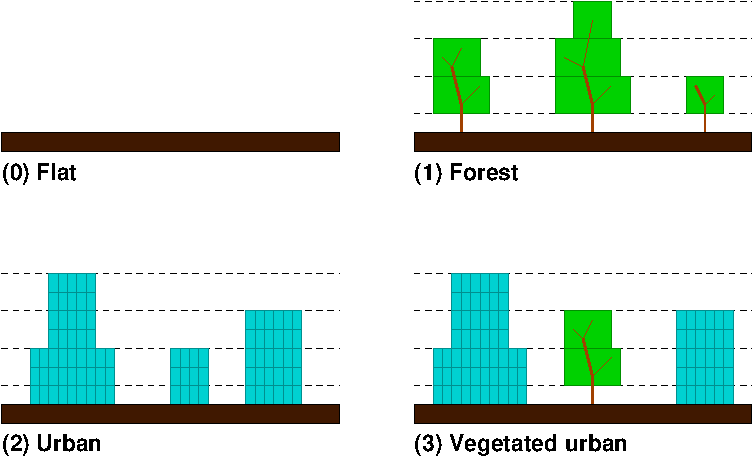
\includegraphics[width=0.75\textwidth]{surface_type_schematic.pdf}}
  \caption{\label{fig:type_schematic}Schematic of the four surfaces
    represented by the \code{surface\_type} variable provided in the
    \spsurf\ input file (see Table \ref{tab:invar}).}
\end{figure}

The output netCDF file contains the typical set of broadband fluxes
and absorption rates listed in Table \ref{tab:outvar}. If you need
them spectrally resolved (using the input spectral discretization)
then set the \code{radsurf\_config} namelist variable
\code{do\_spectral} to \code{true} and the same variables will be
output but with the prefix \code{spectral\_}.




\begin{center}
\tablesetup
\begin{longtable}{llLp{7cm}}%
\caption{\label{tab:outvar}Variables contained in the output netCDF
  file from \spsurf.  All fluxes (or irradiances) and absorption rates
  have units of W~m$^{-2}$, but note that this is power per unit area
  of the \emph{entire domain}, not per unit area of a specific facet
  type.  `Net' fluxes are defined as the flux into a facet type (or downward) minus the
  flux out of a facet type (or upward).}\\
%
\hline
Variable & Dimensions & Description\\
\hline
\codetab{height} & \codetab{col, layer\_int} & Height of layer interfaces above ground (m)\\
\codetab{ground\_flux\_dn\_sw} & \codetab{col} & Downwelling shortwave flux into the ground \\
\codetab{ground\_flux\_net\_sw} & \codetab{col} & Net shortwave flux into the ground\\
\codetab{ground\_flux\_dn\_direct\_sw} & \codetab{col} & Direct downwelling shortwave flux into the ground\\
\codetab{top\_flux\_dn\_sw} & \codetab{col} & Top-of-canopy downwelling shortwave flux\\
\codetab{top\_flux\_net\_sw} & \codetab{col} & Top-of-canopy net shortwave flux\\
\codetab{top\_flux\_dn\_direct\_sw} & \codetab{col} & Top-of-canopy direct downwelling shortwave flux\\
\codetab{roof\_flux\_in\_sw} & \codetab{col, layer} & Shortwave flux into roofs \\
\codetab{roof\_flux\_net\_sw} & \codetab{col, layer} & Net shortwave flux into roofs\\
\codetab{wall\_flux\_in\_sw} & \codetab{col, layer} & Shortwave flux into walls\\
\codetab{wall\_flux\_net\_sw} & \codetab{col, layer} & Net shortwave flux into walls\\
\codetab{clear\_air\_absorption\_sw} & \codetab{col, layer} & Shortwave absorption rate in clear-air part of layer\\
\codetab{veg\_absorption\_sw} & \codetab{col, layer} & Shortwave absorption rate by leaves\\
\codetab{veg\_air\_absorption\_sw} & \codetab{col, layer} & Shortwave absorption rate by air in vegetated part of layer\\
\codetab{ground\_flux\_dn\_lw} & \codetab{col} & Downwelling longwave flux into the ground\\
\codetab{ground\_flux\_net\_lw} & \codetab{col} & Net longwave flux into the ground\\
\codetab{top\_flux\_dn\_lw} & \codetab{col} & Top-of-canopy donwelling longwave flux\\
\codetab{top\_flux\_net\_lw} & \codetab{col} & Top-of-canopy net longwave flux\\
\codetab{roof\_flux\_in\_lw} & \codetab{col, layer} & Longwave flux into roofs\\
\codetab{roof\_flux\_net\_lw} & \codetab{col, layer} & Net longwave flux into roofs\\
\codetab{wall\_flux\_in\_lw} & \codetab{col, layer} & Longwave flux into walls\\
\codetab{wall\_flux\_net\_lw} & \codetab{col, layer} & Net flux into walls\\
\codetab{clear\_air\_absorption\_lw} & \codetab{col, layer} & Net longwave absorption rate in clear-air part of layer\\
\codetab{veg\_absorption\_lw} & \codetab{col, layer} & Net longwave absorption rate by leaves\\
\codetab{veg\_air\_absorption\_lw} & \codetab{col, layer} & Net longwave absorption rate by air in vegetated part of layer\\
\hline
\end{longtable}
\end{center}


\section{Configuring the \spsurf\ algorithm}
\label{sec:nam_radsurf}
The detailed settings of \spsurf\ are configured using the
\code{radsurf} namelist in the namelist file provided as the first
command-line argument to the \code{spartacus\_surface} executable. The
available namelist parameters are listed in Table
\ref{tab:nam_radsurf}.

%\newcommand{\namedef}{3}{\code{#1} & #2 & #3\\}

%\begin{table}
\begin{center}
\tablesetup
%\begin{longtable}{lc>{\raggedright}p{5cm}>{\raggedright}p{5cm}}
%\begin{longtable}{lXLp{4cm}Lp{5.5cm}}
\begin{longtable}{lXlLp{5.5cm}}
%
\caption{\label{tab:nam_radsurf}Options for the \code{radsurf}
  namelist that configures \spsurf\ algorithm. The type of each
  parameter can be inferred from its name: logicals begin with
  \code{do\_} or \code{use\_}, integers start with \code{i\_} or
  \code{n\_}, strings end with \code{\_name}, and all other parameters
  are real numbers.}\\
%
\hline
Parameter & Type & \textbf{Default}, other values & Description\\
\hline
%\namedef{do_sw}{\codetab{true},\codetab{false}}{Run the shortwave scheme?}
\multicolumn{4}{l}{\emph{General}}\\
\codetab{do\_sw} & L & \codetabemph{true} & Compute shortwave fluxes?\\
\codetab{do\_lw} & L & \codetabemph{true} & Compute longwave fluxes?\\
\codetab{do\_vegetation} & L & \codetabemph{true} & Will vegetation be represented? \\
\codetab{do\_urban} & L & \codetabemph{true} & Will urban areas be represented? \\
\codetab{use\_sw\_direct\_albedo} & L & \codetabemph{false} & Specify ground and roof albedos separately for direct solar radiation? \\
\codetab{min\_vegetation\_fraction} & R & \codetabemph{10$^{-6}$} & Minimum area fraction below which a region is removed completely\\
\hline
\multicolumn{4}{l}{\emph{Options specific to forest tiles}}\\
\codetab{n\_vegetation\_region\_forest} & I & \codetabemph{1}, \code{2} & Number of regions used to describe vegetation (2 needed for heterogeneity)\\
\codetab{n\_stream\_sw\_forest} & I & \codetabemph{4} & Streams per hemisphere to describe diffuse shortwave radiation\\
\codetab{n\_stream\_sw\_forest} & I & \codetabemph{4} & Streams per hemisphere to describe longwave radiation\\
\codetab{use\_symmetric\_vegetation\_scale\_forest} & L & \codetabemph{true} & Compute vegetation perimeter length using Eq.\ 20 of \cite{Hogan+2018}? Otherwise Eq.\ 19\\
\codetab{vegetation\_isolation\_factor\_forest} & R & \codetabemph{0.0}, \code{0.0}--\code{1.0} & Dense vegetation region is (0.0) embedded within sparse region or (1.0) in physically isolated regions\\
\hline
\multicolumn{4}{l}{\emph{Options specific to urban tiles}}\\
\codetab{n\_vegetation\_region\_urban} & I & \codetabemph{1}, \code{2} & Number of regions used to describe vegetation (2 needed for heterogeneity)\\
\codetab{n\_stream\_sw\_urban} & I & \codetabemph{4} & Streams per hemisphere to describe diffuse shortwave radiation\\
\codetab{n\_stream\_sw\_urban} & I & \codetabemph{4} & Streams per hemisphere to describe longwave radiation\\
\codetab{use\_symmetric\_vegetation\_scale\_urban} & L & \codetabemph{true} & Compute vegetation perimeter length using Eq.\ 20 of \cite{Hogan+2018}? Otherwise Eq.\ 19\\
\codetab{vegetation\_isolation\_factor\_urban} & R & \codetabemph{0.0}, \code{0.0}--\code{1.0} & Dense vegetation region is (0.0) embedded within sparse region or (1.0) in physically isolated regions\\
%\hline
%\multicolumn{4}{l}{\emph{Gas and aerosol optics}}\\
%\codetab
\hline
% To be added:
%     &  do_canopy_gases_sw, do_canopy_gases_lw, 
\end{longtable}
\end{center}
%\end{table}

The number of streams can be any positive integer, but note that this
is the number of quadrature points that the radiation field is divided
into \emph{per hemisphere}, so a value of 4 corresponds to an
`8-stream scheme' in the convention that all possible directions are
considered.  Larger values give more accuracy at greater computational
cost, but as shown by \cite{Hogan2019b}, there is little change in the
results above a value of 4.

The other parameters in Table \ref{tab:nam_radsurf} allow the
treatment of vegetation to be fine tuned. If the number of vegetation
regions is 1 then the trees are represented as in
Fig.\ \ref{fig:type_schematic}, with a single vegetation extinction
coefficient per layer.  In order to represent horizontal heterogeneity
within tree crowns, a value of 2 should be selected, resulting in the
representation in Fig.\ \ref{fig:isolation_schematic}. The
\code{vegetation\_isolation\_factor\_*} parameters describe the
contact between the clear region and the two vegetated regions in each
layer, with the extremes being 0.0 in which the denser vegetation
region is completely embedded in the sparser region \cite[the
  assumption used by][]{Hogan+2018}, and 1.0 in which the dense and
sparse regions form unconnected tree crowns.

\begin{figure}[b!]
  \centerline{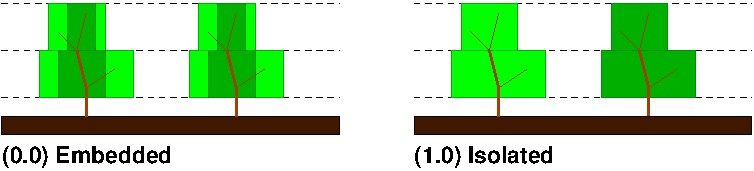
\includegraphics[width=0.75\textwidth]{isolation_schematic.pdf}}
  \caption{\label{fig:isolation_schematic}Schematic illustrating how
    the \code{vegetation\_isolation\_factor\_*} parameters in Table
    \ref{tab:nam_radsurf} describe the contact between the clear-air
    region and the two vegetated regions in each layer.}
\end{figure}

\spsurf\ assumes that the rate of lateral exchange of radiation
between the clear and vegetated regions is proportional to the
normalized perimeter length, $L$, separating the vegetation and clear
regions, i.e.\ the perimeter length divided by the horizontal area of
the domain. This variable has units of m$^{-1}$ and is a strong
function of vegetation fraction, so it is more convenient for models to
parameterize the horizontal size of typical tree crowns, as expressed
by the \code{vegetation\_scale} input variable in Table
\ref{tab:invar}. The \code{use\_symmetric\_vegetation\_scale\_*}
parameters determine how this scale is used to compute $L$.  If a
symmetric vegetation scale is selected then Eq.\ 20 of
\cite{Hogan+2018} is used:
%
\begin{equation}
  L=4v(1-v)/S,\label{eq:S}
\end{equation}
%
where $v$ is the vegetation fraction and $S$ is the vegetation scale.
In this case, as the vegetation fraction approaches one, the
normalized perimeter approaches zero, indicating that the tree crowns
effectively merge. If \code{use\_symmetric\_vegetation\_scale\_*} is
\code{false} then Eq.\ 19 of \cite{Hogan+2018} is used:
%
\begin{equation}
  L=4v/D,\label{eq:D}
\end{equation}
%
where this time \code{vegetation\_scale} is interpreted as the
effective crown diameter, $D$. This has the property that $L$
approaches a constant value as the vegetation fraction approaches one,
which could be thought of as the property of \emph{crown shyness}
exhibited by some forest canopies.

The \code{building\_scale} input variable in Table \ref{tab:invar} is
always interpreted as an effective building diameter, i.e.\ the code
uses (\ref{eq:D}) to convert to the normalized building perimeter
length in each layer, $L$, given the building fraction $v$.

\section{Configuring the offline package}
\label{sec:nam_radsurf_config}
In addition to the namelist parameters described in section
\ref{sec:nam_radsurf} an additional set of parameters are available in
the \code{radsurf\_config} namelist that are specific to the offline
version of \spsurf\ and are listed in Table
\ref{tab:nam_radsurf_config}. In general if these parameters are
present in the namelist then they will override the corresponding
variable provided in the input file.

\begin{center}
\tablesetup
\begin{longtable}{ll}
%
\caption{\label{tab:nam_radsurf_config}Options for the
  \code{radsurf\_config} namelist that configures additional aspects
  of the offline radiation scheme. All entries must be scalars. If an
  override parameter is present then usually it need not be included
  in the input file.}\\
%
\hline
Parameter & Description\\
\hline
\multicolumn{2}{l}{\emph{Execution control}}\\
\codetab{nrepeat}  & Number of times to repeat, for benchmarking\\
\codetab{istartcol} & Start at specified input column (1 based)\\
\codetab{iendcol} & End at specified input column (1 based)\\
\codetab{iverbose} & Verbosity in offline setup (default 2)\\
\codetab{do\_parallel} & Use OpenMP parallelism? (default \codetab{true})\\
\codetab{nblocksize} & Number of columns per block when using OpenMP\\
\codetab{do\_conservation\_check} & Check final energy balance for each column\\
\hline
\multicolumn{2}{l}{\emph{Override input variables}}\\
\codetab{cos\_solar\_zenith\_angle} & Override cosine of solar zenith angle\\
\codetab{ground\_sw\_albedo} & Override shortwave albedo of ground\\
\codetab{roof\_sw\_albedo} & Override shortwave albedo of roofs\\
\codetab{wall\_sw\_albedo} & Override shortwave albedo of walls\\
\codetab{ground\_lw\_emissivity} & Override longwave emissivity of ground\\
\codetab{roof\_lw\_emissivity} & Override longwave emissivity of roofs\\
\codetab{wall\_lw\_emissivity} & Override longwave emissivity of walls\\
\codetab{vegetation\_fraction} & Override vegetation fraction \\
\codetab{vegetation\_extinction} & Override vegetation extinction coefficient (m$^{-1}$)\\
\codetab{vegetation\_fsd} & Override vegetation fractional standard deviation of extinction\\
\codetab{vegetation\_sw\_ssa} & Override vegetation shortwave single scattering albedo \\
\codetab{vegetation\_lw\_ssa} & Override vegetation longwave single scattering albedo \\
\codetab{top\_flux\_dn\_sw} & Override top-of-canopy downwelling shortwave flux (W~m$^{-2}$)\\
\codetab{top\_flux\_dn\_direct\_sw} & Override top-of-canopy downwelling direct shortwave flux (W~m$^{-2}$)\\
\codetab{top\_flux\_dn\_lw} & Override top-of-canopy downwelling longwave flux (W~m$^{-2}$)\\
\hline
\end{longtable}
\end{center}

\section{Checking the configuration}
\label{sec:checking}
When \code{spartacus\_surface} is run, it outputs to the screen a
summary of the configuration options, with the level of detail
controled by the \code{radsurf\_config} namelist parameter
\code{iverbose}. This can be used to check that \spsurf\ has been
configured as intended.  The following is an example from the default
test in the \code{test/simple} directory, in the case of
\code{iverbose=2}:

\footnotesize
\begin{verbatim}
------------------ OFFLINE SPARTACUS-SURFACE RADIATION SCHEME ------------------
Copyright (C) 2019-2020 European Centre for Medium-Range Weather Forecasts
Contact: Robin Hogan (r.j.hogan@ecmwf.int)
Floating-point precision: double
General settings:
  Represent vegetation ON                 (do_vegetation=T)
  Represent urban areas ON                (do_urban=T)
  Do shortwave (SW) calculations ON       (do_sw=T)
  Do longwave (LW) calculations ON        (do_sw=T)
  Number of SW spectral intervals = 1     (nsw)
  Number of LW spectral intervals = 1     (nlw)
  Minimum vegetation fraction = .100E-05  (min_vegetation_fraction)
Settings for forests:
  Number of vegetation regions = 2        (n_vegetation_region_forest)
  Use symmetric vegetation scale ON       (use_symmetric_vegetation_scale_forest=T)
  Vegetation isolation factor = 0.00      (vegetation_isolation_factor_forest)
  SW diffuse streams per hemisphere = 2   (n_stream_sw_forest)
  LW streams per hemisphere = 2           (n_stream_lw_forest)
Settings for urban areas:
  Number of vegetation regions = 2        (n_vegetation_region_urban)
  Use symmetric vegetation scale ON       (use_symmetric_vegetation_scale_urban=T)
  Vegetation isolation factor = 0.00      (vegetation_isolation_factor_urban)
  SW diffuse streams per hemisphere = 2   (n_stream_sw_urban)
  LW streams per hemisphere = 2           (n_stream_lw_urban)
Reading NetCDF file test_surfaces_in.nc
  Overriding cosine of the solar zenith angle with  0.500    
  Overriding vegetation extinction with  0.250    
  Setting temperature of clear-air and air in vegetation to air_temperature
  Setting vegetation temperature equal to air temperature
  Assuming roof albedo to direct albedo is the same as to diffuse
  Assuming wall reflection is Lambertian (no specular component)
    1: Flat
    2: Forest,            2 layers, 2 diffuse streams per hemisphere, 3 regions
    3: Unvegetated urban, 2 layers, 2 diffuse streams per hemisphere, 1 region
    4: Vegetated urban,   2 layers, 2 diffuse streams per hemisphere, 3 regions
Direct shortwave budget
Layer   Ground      Air     Wall     Roof      Veg  Air-veg      Top   Residual
    1  320.000    0.000    0.000    0.000    0.000    0.000  320.000  0.000E+00
    2   87.441    0.000    0.000    0.000  293.893    0.000  381.334  0.568E-13
    3   51.015    0.000  185.652  119.081    0.000    0.000  355.748 -0.568E-13
    4   25.686    0.000  163.389  119.057   51.620    0.000  359.752  0.000E+00
Diffuse shortwave budget
Layer   Ground      Air     Wall     Roof      Veg  Air-veg      Top   Residual
    1   80.000    0.000    0.000    0.000    0.000    0.000   80.000  0.000E+00
    2   27.565    0.000    0.000    0.000   67.146    0.000   94.710  0.000E+00
    3   20.203    0.000   37.465   30.846    0.000    0.000   88.514  0.000E+00
    4   13.199    0.000   33.583   30.840   12.105    0.000   89.726 -0.142E-13
Internal longwave budget
Layer   Ground      Air     Wall     Roof      Veg  Air-veg      Top   Residual
    1 -328.035    0.000    0.000    0.000    0.000    0.000 -328.035  0.000E+00
    2 -327.647    0.031    0.000    0.000  216.819    0.011 -110.785  0.847E-05
    3  -80.093   -0.158 -138.486 -125.417    0.000    0.000 -344.211  0.569E-01
    4  -55.546   -0.151 -130.312 -125.423  -32.158   -0.002 -343.627  0.351E-01
Incoming longwave budget
Layer   Ground      Air     Wall     Roof      Veg  Air-veg      Top   Residual
    1  263.855    0.000    0.000    0.000    0.000    0.000  263.855  0.000E+00
    2   89.108    0.029    0.000    0.000  198.716    0.010  287.868 -0.416E-02
    3   64.432    0.157  111.365  100.876    0.000    0.000  276.877 -0.462E-01
    4   41.886    0.146  101.133  100.871   34.728    0.002  278.796 -0.287E-01
Writing NetCDF file test_surfaces_out.nc
--------------------------------------------------------------------------------

\end{verbatim}
\normalsize

\section{Incorporating \spsurf\ into another program}
\label{sec:api}
%\label{ch:api}
\spsurf\ is primarily a software library that is designed to be called
from within a larger program such as an atmospheric model.  The
library is written entirely using Fortran modules, and you will need
all the Fortran source files in the \code{utilities}, \code{radtool}
and \code{radsurf} directories.  The
\code{utilities/radiation\_io.F90} file provides the \code{nulout}
unit for logging messages and the \code{radiation\_abort} routine for
exiting if an error occurs.  This file will likely need to be
rewritten for your model, for example to ensure appropriate clean-up
after an anomalous abort.

\iffalse
\begin{lstlisting}
 ! Integers
 ncol                 ! Number of columns
 ntotlay              ! Total number of layers
  
 ! Allocatable integer vectors of length "ncol"
 nlay                 ! Number of layers in column
 istartlay            ! Index of first layer
 i_representation     ! Surface type (0-4)
 
 ! Allocatable real vectors of length "ncol"
 dz                   ! Layer thickness (m)
 cos_sza              ! Cosine of solar zenith angle
 ground_temperature   ! Ground temperature (K)
 
 ! Allocatable real vectors of length "ntotlay"
 roof_temperature, wall_temperature, clear_air_temperature, building_fraction, veg_fraction,
 building_scale, veg_scale, veg_ext, veg_fsd, veg_contact_fraction
\end{lstlisting}
\fi

\spsurf\ adopts a strict policy of no global variables and no
variables in modules (which are really a type of global
variable). Therefore, information is passed to and from routines only
via the arguments to those routines.  This includes configuration
information, which is stored in a \code{config\_type} object from the
\code{radsurf\_config} module. As part of the initialization stage of
the atmospheric model, such an object should be created, and will
later be passed to the routine that performs the radiative transfer. A
configuration object is created as follows:
%
\begin{lstlisting}
 use radsurf_config, only : config_type ! Read module defining configuration type
 type(config_type) :: config            ! Create a configuration object
 ! ...optionally set some default values - see radsurf/radsurf_config.F90...
 call config%read(namelist_file_name)   ! Read configuration information from a namelist file
 call config%consolidate()              ! Perform any additional configuration steps needed
\end{lstlisting}

Performing radiative transfer on a set of \code{ncol} surface canopy
profiles is carried out in two parts. In the first part, the geometric
and spectral properties of the canopies are used to compute (1) the
top-of-canopy properties presented to the atmosphere above such as
spectral albedo and upward longwave emission, and (2) fluxes within
the canopy that are normalized with respect to downwelling shortwave
and longwave fluxes at the top-of-canopy. It is envisaged that after
this step, the top-of-canopy properties presented to the atmosphere
are used as boundary conditions for a full atmospheric radiative
transfer calculation.  One of the outputs of such a calculation is the
downwelling spectral shortwave and longwave fluxes at
top-of-canopy. The second (much simpler) part of the interface to
\spsurf\ involves scaling the normalized fluxes computed in the first
step to obtain the absolute fluxes within the canopy, including net
fluxes into ground, roofs, walls and vegetation.  These fluxes and
heating rates can then be used by a canopy energy balance model.

The first part involves calling the \code{radsurf} routine, which
takes as arguments a number of objects.  The input description of the
canopy is in the form of three Fortran derived types: the
\code{canopy\_properties\_type} describes the wavelength-independent
properties of the canopy, and the
\code{sw\_spectral\_properties\_type} and
\code{lw\_spectral\_properties\_type} describe the shortwave and
longwave spectral properties.  Each object describes \code{ncol}
surface `columns' to be treated independently; each column could
correspond to an atmospheric model column, or alternatively may
represent multiply `tiles' underlying one or more atmospheric columns.

The arrays in the \code{canopy\_properties\_type} could have been
dimensioned \code{nmaxlay}$\times$\code{ncol}, where \code{nmaxlay} is
the maximum number of layers in any of the individual columns.
However, it is recognised that in a global model many or even most of
the columns would be treated as `flat' (type 0 in
Fig.\ \ref{fig:type_schematic}) and many layers would be unused.
Therefore the arrays in these objects use a `packed' representation,
explained by considering some of the elements of
\code{canopy\_properties\_type}:
\begin{lstlisting}
 ! Integers
 ncol                ! Number of columns
 ntotlay             ! Total number of layers

 ! Allocatable integer vectors of length "ncol"
 nlay                ! Number of layers in column (can be 0)
 istartlay           ! Index to first layer of the column
 i_representation    ! Surface type (0-3)

 ! Allocatable real vectors of length "ncol"
 cos_sza, ground_temperature

 ! Allocatable real vectors of length "ntotlay"
 roof_temperature, wall_temperature, building_fraction, veg_fraction...
\end{lstlisting}
It can be seen that the variables describing properties as a function
of height (e.g. wall temperature) are vectors of dimension
\code{ntotlay}, expressing the total number of layers in this block of
columns. The integer vectors \code{nlay} and \code{istartlay} enable
the range of elements corresponding to the layers of a particular
column to be identified.  The \code{sw\_spectral\_properties\_type}
and \code{lw\_spectral\_properties\_type} are packed similarly, except
that each array has an additional \code{nspec} dimension expressing
the number of shortwave or longwave spectral intervals.

Preparation of these three objects can be done as follows:
%
\begin{lstlisting}
 ! Read modules defining the three derived types
 use radsurf_canopy_properties,      only : canopy_properties_type
 use radsurf_sw_spectral_properties, only : sw_spectral_properties_type
 use radsurf_lw_spectral_properties, only : lw_spectral_properties_type

 ! Declare instances of these types
 type(canopy_properties_type)      :: canopy_props
 type(sw_spectral_properties_type) :: sw_spectral_props
 type(lw_spectral_properties_type) :: lw_spectral_props

 ! Allocate canopy properties given existing configuration object "config", number of columns 
 ! "ncol", total number of layers "ntotlay" and number of shortwave and longwave spectral
 ! intervals "nsw" and "nlw":
 call      canopy_props%allocate(config, ncol, ntotlay)
 call sw_spectral_props%allocate(config, ncol, ntotlay, nsw)
 call lw_spectral_props%allocate(config, ncol, ntotlay, nlw)
\end{lstlisting}
Subsequent code would then populate the arrays within these three
objects using data from the host model (consult the files
\code{radsurf\_canopy\_properties.F90},
\code{radsurf\_sw\_spectral\_properties.F90} and
\code{radsurf\_lw\_spectral\_properties.F90} for precise contents of
these arrays).  Note that the offline driver program
\code{driver/spartacus\_surface\_driver.F90} does not use these
\code{allocate} type-bound procedures, but rather populates the arrays
within the objects directly using the contents of the input netCDF
file.

We also need to prepare objects to hold the output from the
\code{radsurf} routine:
\begin{lstlisting}
 ! Read modules defining the relevant derived types
 use radsurf_boundary_conds_out,     only : boundary_conds_out_type
 use radsurf_canopy_flux,            only : canopy_flux_type

 ! Declare an object holding the top-of-canopy boundary conditions presented to the atmosphere
 ! above
 type(boundary_conds_out_type) :: bc_out 
 ! Declare canopy flux components: the first three contain the fluxes and net absorption rates
 ! within the canopy normalized by the shortwave-diffuse, shortwave-direct and longwave
 ! downwelling flux at top-of-canopy. The fourth contains the same but purely due to internal 
 ! longwave emission within the canopy
 type(canopy_flux_type)        :: sw_norm_diff, sw_norm_dir, lw_norm, lw_internal 

 ! Allocate these objects, noting that the shortwave objects use internal arrays to also store 
 ! direct fluxes, not needed in the longwave
 call       bc_out%allocate(ncol, nsw, nlw)
 call sw_norm_diff%allocate(config, ncol, ntotlay, nsw, use_direct=.true.)
 call  sw_norm_dir%allocate(config, ncol, ntotlay, nsw, use_direct=.true.)
 call  lw_internal%allocate(config, ncol, ntotlay, nlw, use_direct=.false.)
 call      lw_norm%allocate(config, ncol, ntotlay, nlw, use_direct=.false.)

 ! Optionally set all fluxes to zero
 call  sw_norm_dir%zero_all()
 call sw_norm_diff%zero_all()
 call  lw_internal%zero_all()
 call      lw_norm%zero_all()
\end{lstlisting}

We are now in a position to call the \code{radsurf} routine:
\begin{lstlisting}
 ! Read module defining the radsurf routine
 use radsurf_interface, only : radsurf

 ! ...prepare the objects to pass to radsurf...

 ! Call the SPARTACUS-Surface radiation scheme
 call radsurf(config, canopy_props, sw_spectral_props, lw_spectral_props, & ! Inputs
      &       bc_out, &                                                     ! Outputs
      &       istartcol, iendcol, &                                         ! Optional inputs
      &       sw_norm_dir, sw_norm_diff, lw_internal, lw_norm)              ! Optional outputs
\end{lstlisting}
Optionally, a call to \code{radsurf} may specify the range of columns
to process via \code{istartcol} and \code{iendcol}.  This is useful
for OpenMP parallelization: if the objects contain a large number of
columns then \code{radsurf} can be called simultaneously by mutliple
threads, each thread being instructed to work on a different range of
columns.  This is done by the offline \spsurf\ driver. The final four
canopy flux objects are marked as `optional' because the \code{config}
object may have specified to only perform shortwave or longwave
radiative transfer, in which case only two such output objects would
be needed.

The \code{boundary\_conds\_out\_type} is fairly small, containing four
arrays. The arrays \code{sw\_albedo} and \code{sw\_albedo\_dir} are
the shortwave spectral albedo at top-of-canopy presented to incoming
diffuse and direct solar radiation, and are dimensioned
\code{nsw}$\times$\code{ncol}. The arrays \code{lw\_emissivity} and
\code{lw\_emission} are the top-of-canopy longwave spectral emissivity
and upward emission (in W~m$^{-2}$), dimensioned
\code{nlw}$\times$\code{ncol}.

After the atmospheric radiative transfer calculation has completed
using these arrays as boundary conditions, we need to use the
downwelling fluxes at top-of-canopy to scale the normalized canopy
fluxes. 
\begin{lstlisting}
 ! Declare objects to contain total (unnormalized) canopy fluxes
 type(canopy_flux_type) :: lw_flux, sw_flux

 ! Allocate these objects
 call sw_flux%allocate(config, ncol, ntotlay, nsw, use_direct=.true.)
 call lw_flux%allocate(config, ncol, ntotlay, nlw, use_direct=.false.)

 ! Suppose the atmospheric radiative transfer scheme has provided three arrays of spectral
 ! downwelling radiation at top of canopy, top_flux_dn_diffuse_sw(nsw,ncol),
 ! top_flux_dn_direct_sw(nsw,ncol) and top_flux_dn_lw(nlw,ncol), we can use them to scale
 ! the normalized shortwave and longwave canopy fluxes, also taking as input the number of
 ! layers stored in each column, canopy_props%nlay
 call sw_norm_diff%scale(canopy_props%nlay, top_flux_dn_diffuse_sw)
 call  sw_norm_dir%scale(canopy_props%nlay, top_flux_dn_direct_sw)
 call      lw_norm%scale(canopy_props%nlay, top_flux_dn_lw)

 ! Finally, sum the two contributions in each spectral region to obtain total (unnormalized)
 ! canopy fluxes
 call sw_flux%sum(sw_norm_dir, sw_norm_diff)
 call lw_flux%sum(lw_internal, lw_norm)
\end{lstlisting}
The contents of \code{sw\_flux} and \code{lw\_flux} are then available
to use in a canopy energy balance scheme.  See
\code{radsurf\_radsurf\_canopy\_flux.F90} for the precise contents of
these objects. Note that at this stage they are still in the same
spectral intervals as used by the \spsurf\ calculation.  In the
shortwave this is useful as it enables the photosynthetically active
part of the spectral absorption by vegetation to be computed.

\emph{Further development is still needed on the spectral aspect of
  \spsurf.  It is expected that in the shortwave, the radiation
  calculations will all be performed in the user-specified spectral
  intervals, and atmospheric extinction will either be ignored or it
  will be left to the user to provide atmospheric extinction
  coefficients, especially due to aerosols. It ought to be reasonable
  to neglect gas absorption and Rayleigh scattering since the Rayleigh
  optical depth is small through the limited depth of a surface
  canopy, and in the parts of the near-infrared spectrum where the
  gaseous absorpion is large, little solar radiation is likely to
  penetrate down through the atmosphere to the top of the canopy.}

\emph{In the longwave, there will need to be a mechanism to treat
  gaseous absorption given its importance \cite[]{Hogan2019b}. This
  could be implemented by mapping the user-specified longwave spectral
  intervals on to a larger number of intervals suitable for longwave
  radiative transfer and running \spsurf\ at this spectral resolution.
  The larger number of intervals could then be passed to the
  atmospheric longwave radiative transfer.  For the canopy energy
  balance model, only the broadband longwave fluxes are likely to be
  of interest, which could be computed by simply summing the fluxes along
  the \code{nlw} dimension.}

\section{License and copyright}
The SPARTACUS-Surface software is copyright \copyright\ 2019-- ECMWF. This
software is licensed under the terms of the Apache Licence Version 2.0
which can be obtained at
\url{http://www.apache.org/licenses/LICENSE-2.0}.  In applying this
licence, ECMWF does not waive the privileges and immunities granted to
it by virtue of its status as an intergovernmental organisation nor
does it submit to any jurisdiction.

\begin{thebibliography}{00}
\markright{References}
%
\harvarditem{Hogan}{2019a}{Hogan2019a}Hogan, R. J., 2019a: An
exponential model of urban geometry for use in radiative transfer
applications. \textit{Boundary-Layer Meteorol.,} \textbf{170,}
357--472.
%
\harvarditem{Hogan}{2019b}{Hogan2019b}Hogan, R. J., 2019b: Flexible
treatment of radiative transfer in complex urban canopies for use in
weather and climate models. \textit{Boundary-Layer Meteorol.,}
\textbf{173,} 53-78.
%
\harvarditem{Hogan et~al.}{2018}{Hogan+2018}Hogan, R. J., T. Quaife
and R. Braghiere, 2018: Fast matrix treatment of 3-D radiative
transfer in vegetation canopies: SPARTACUS-Vegetation
1.1. \textit{Geosci.\ Model Dev.,} \textbf{11,} 339-350.
%

%\harvarditem{Fielding~et~al.}{2020}{Fielding+2020}Fielding, M. D.,
%S. A. K. Sch\"afer, R. J. Hogan and R. M. Forbes, 2020: Encapsulating
%cloud geometry for 3D radiative transfer and cloud turbulent mixing
%parameterizations. \emph{To be submitted to Q. J. R. Meteorol.\ Soc.}
%
%\harvarditem{Hogan and Bozzo}{2018}{Hogan+2018}Hogan, R. J., and
%A. Bozzo, 2018: A flexible radiation scheme for the ECMWF
%model. \textit{J. Adv.\ Model.\ Earth Syst.,} \textbf{10,}
%doi:10.1029/2018MS001364.
%
\harvarditem{Hogan~et~al.}{2016}{Hogan+2016}Hogan, R. J.,
S. A. K. Sch\"afer, C. Klinger, J.-C. Chiu and B. Mayer, 2016:
Representing 3D cloud-radiation effects in two-stream schemes:
2. Matrix formulation and broadband
evaluation. \textit{J. Geophys.\ Res.,} \textbf{121,} 8583--8599.
%
%\harvarditem{Hogan~et~al.}{2019}{Hogan+2019}Hogan, R. J.,
%M. D. Fielding, H. W. Barker, N. Villefranque and S. A. K. Sch\"afer,
%2019: Entrapment: An important mechanism to explain the shortwave 3D
%radiative effect of clouds. \textit{J. Atmos.\ Sci.,} \textbf{76,}
%2123--2141.
%
\harvarditem{Shonk and Hogan}{2008}{Shonk+2008}Shonk, J. K. P., and
R. J. Hogan, 2008: Tripleclouds: an efficient method for representing
horizontal cloud inhomogeneity in 1D radiation schemes by using three
regions at each height. \textit{J. Climate,} \textbf{21,} 2352--2370.
%
\harvarditem{Stamnes et~al.}{1988}{Stamnes+1988}Stamnes K.,
S. C. Tsay, W. Wiscombe and K. Jayaweera, 1988: Numerically stable
algorithm for discrete-ordinate-method radiative transfer in multiple
scattering and emitting layered media. \textit{Appl.\ Opt.,}
\textbf{27,} 2502--2509.
\end{thebibliography}
\end{document}
